% Propósito: mostrar que la directividad redistribuye una potencia total sin
% crear energía y que Q compara intensidades a igual potencia y distancia.
% Origen: Q(theta,phi)=I(r,theta,phi)/(W/(4 pi r^2)), ecuación
% \eqref{eq:u4-factor-directividad}. Los patrones son esquemáticos y no
% corresponden a un transductor ni a una frecuencia medidos.
% Descripción accesible: a la izquierda, una sección polar circular representa
% una fuente omnidireccional. A la derecha, una sección con un lóbulo principal
% hacia la derecha representa una fuente direccional. En una dirección dada y
% a igual potencia y distancia, Q compara la intensidad direccional con la
% intensidad de la fuente omnidireccional.
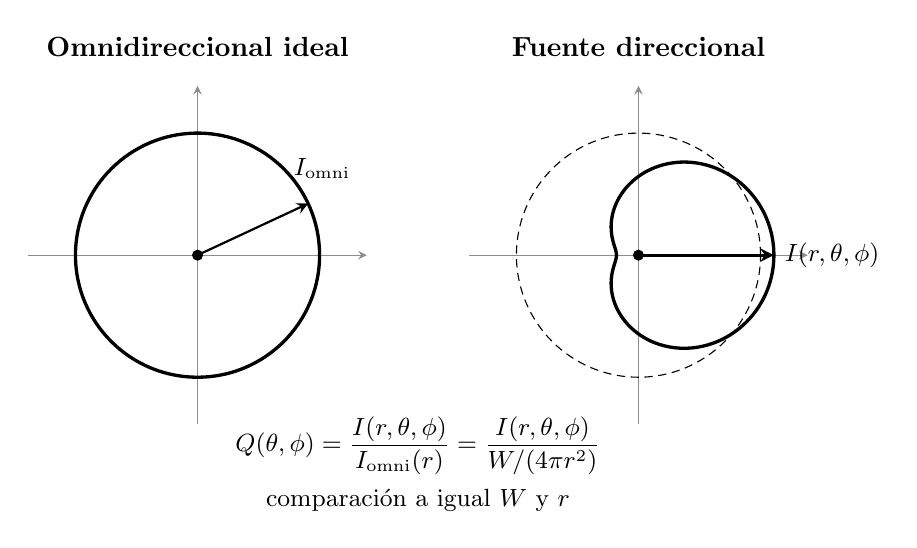
\begin{tikzpicture}[font=\small,>=stealth,x=1cm,y=1cm]
    \coordinate (O) at (2.95,2.75);
    \coordinate (D) at (8.55,2.75);

    \node[font=\bfseries] at (2.95,5.40) {Omnidireccional ideal};
    \node[font=\bfseries] at (8.55,5.40) {Fuente direccional};

    \draw[->,black!45] (0.80,2.75) -- (5.10,2.75);
    \draw[->,black!45] (2.95,0.60) -- (2.95,4.90);
    \draw[->,black!45] (6.40,2.75) -- (10.70,2.75);
    \draw[->,black!45] (8.55,0.60) -- (8.55,4.90);
    \fill (O) circle (2pt);
    \fill (D) circle (2pt);

    \draw[very thick] (O) circle (1.55cm);
    \node[anchor=west] at (4.05,3.85) {\(I_\mathrm{omni}\)};
    \draw[->,thick] (O) -- ++(25:1.55);

    \draw[very thick,samples=160,domain=0:360,smooth,variable=\a]
        plot ({8.55+(1.00+0.72*cos(\a))*cos(\a)},
              {2.75+(1.00+0.72*cos(\a))*sin(\a)});
    \draw[->,very thick] (D) -- ++(0:1.72)
        node[anchor=west] {\(I(r,\theta,\phi)\)};
    \draw[densely dashed] (D) circle (1.55cm);

    \node[align=center] at (5.75,0.10)
        {\(\displaystyle
          Q(\theta,\phi)
          =\frac{I(r,\theta,\phi)}
                 {I_\mathrm{omni}(r)}
          =\frac{I(r,\theta,\phi)}
                 {W/(4\pi r^2)}\)\\[4pt]
         comparación a igual \(W\) y \(r\)};
\end{tikzpicture}
